\documentclass[tikz,border=10pt]{standalone}
\usepackage{tikz}
\usetikzlibrary{positioning,fit,arrows.meta}
\usepackage{amsmath}

\tikzset{
  mc/.style={draw, minimum width=1.5cm, minimum height=1cm, align=center},
  mylabel/.style={font=\sffamily\footnotesize},
  myarrow/.style={-{Latex[length=3pt]}, thick},
}

\begin{document}
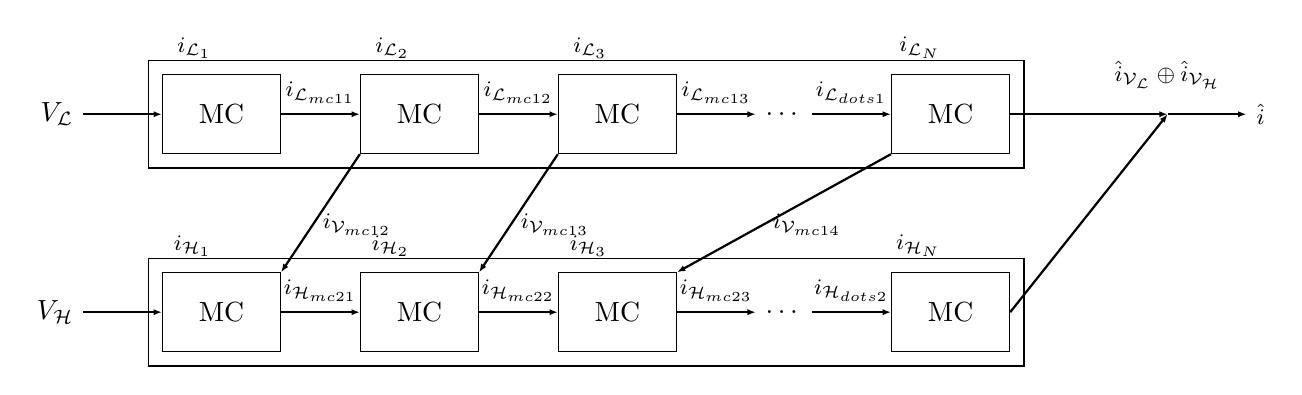
\begin{tikzpicture}[node distance=1.5cm and 1cm]
  % Nodes for top row
  \node[mc] (mc11) {MC};
  \node[mc,right=of mc11] (mc12) {MC};
  \node[mc,right=of mc12] (mc13) {MC};
  \node[right=of mc13] (dots1) {\dots};
  \node[mc,right=of dots1] (mc14) {MC};

  % Nodes for bottom row
  \node[mc,below=of mc11] (mc21) {MC};
  \node[mc,right=of mc21] (mc22) {MC};
  \node[mc,right=of mc22] (mc23) {MC};
  \node[right=of mc23] (dots2) {\dots};
  \node[mc,right=of dots2] (mc24) {MC};

  % Voltage sources
  \node[left=of mc11] (vL) {$V_{\mathcal{L}}$};
  \node[left=of mc21] (vH) {$V_{\mathcal{H}}$};

  % Current labels for top row
  \node[above=2pt of mc11, anchor=south east, mylabel] (iL1) {$i_{\mathcal{L}_1}$};
  \node[above=2pt of mc12, anchor=south east, mylabel] (iL2) {$i_{\mathcal{L}_2}$};
  \node[above=2pt of mc13, anchor=south east, mylabel] (iL3) {$i_{\mathcal{L}_3}$};
  \node[above=2pt of mc14, anchor=south east, mylabel] (iLN) {$i_{\mathcal{L}_N}$};

  % Current labels for bottom row
  \node[above=2pt of mc21, anchor=south east, mylabel] (iH1) {$i_{\mathcal{H}_1}$};
  \node[above=2pt of mc22, anchor=south east, mylabel] (iH2) {$i_{\mathcal{H}_2}$};
  \node[above=2pt of mc23, anchor=south east, mylabel] (iH3) {$i_{\mathcal{H}_3}$};
  \node[above=2pt of mc24, anchor=south east, mylabel] (iHN) {$i_{\mathcal{H}_N}$};

  % Arrows and current labels for top row
  \draw[myarrow] (vL.east) -- (mc11.west) node[midway, above, mylabel] {};
  \foreach \i/\j in {mc11/mc12, mc12/mc13, mc13/dots1, dots1/mc14} {
    \draw[myarrow] (\i.east) -- (\j.west) node[midway, above, mylabel] {$i_{\mathcal{L}_{\i}}$};
  }

  % Arrows and current labels for bottom row
  \draw[myarrow] (vH.east) -- (mc21.west) node[midway, above, mylabel] {};
  \foreach \i/\j in {mc21/mc22, mc22/mc23, mc23/dots2, dots2/mc24} {
    \draw[myarrow] (\i.east) -- (\j.west) node[midway, above, mylabel] {$i_{\mathcal{H}_{\i}}$};
  }

  % Cross connections between rows
  \foreach \i/\j in {mc12/mc21, mc13/mc22, mc14/mc23} {
    \draw[myarrow] (\i.south west) -- (\j.north east) node[pos=0.6, right, mylabel] {$i_{\mathcal{V}_{\i}}$};
  }

  % Summation block
  \coordinate[right=2cm of mc14.east] (sum) {};
  \node[above=0.2cm of sum, mylabel] (sum_label) {$\hat{i}_{\mathcal{V}_{\mathcal{L}}} \oplus \hat{i}_{\mathcal{V}_{\mathcal{H}}}$};
  \draw[-{Latex[length=3pt]}, thick] (mc14.east) -- (sum);
  \draw[-{Latex[length=3pt]}, thick] (mc24.east) -- (sum);
  \draw[-{Latex[length=3pt]}, thick] (sum) -- ++(1cm,0) node[right, mylabel] {$\hat{i}$};

  % Fit boxes around the rows
  \node[draw, fit=(mc11)(mc14), inner sep=5pt] {};
  \node[draw, fit=(mc21)(mc24), inner sep=5pt] {};

\end{tikzpicture}
\end{document}